%-------------------------------------------------
%	Version: 0.0
%	fecha de entrega
%
%-------------------------------------------------

\documentclass[11pt]{report}

%packages
\usepackage{graphicx}
\usepackage{subcaption}

\usepackage[utf8]{inputenc}
\usepackage[spanish, es-nodecimaldot]{babel}
\usepackage{setspace}
\usepackage{ragged2e}

\usepackage{amsmath}
\usepackage{amsthm}
\usepackage{amssymb}
\usepackage{mathtools}
\usepackage{siunitx}

%path donde se encuentran las imagenes
\graphicspath{ {./figuras/} }

%---------------------------------------------------------------
%ABREVIACIONES DE COMANDOS

\theoremstyle{plain}
\newtheorem{thm}{Teorema}[chapter] % reset theorem numbering for each chapter

\theoremstyle{definition}
\newtheorem{defn}[thm]{Definición} % definition numbers are dependent on theorem numbers
\newtheorem{exmp}[thm]{Ejemplo} % same for example numbers

\newcommand{\chaptercontent}{
\section{Basics}
\begin{defn}Here is a new definition.\end{defn}
\begin{thm}Here is a new theorem.\end{thm}
\begin{thm}Here is a new theorem.\end{thm}
\begin{exmp}Here is a good example.\end{exmp}
\subsection{Some tips}
\begin{defn}Here is a new definition.\end{defn}
\section{Advanced stuff}
\begin{defn}Here is a new definition.\end{defn}
\subsection{Warnings}
\begin{defn}Here is a new definition.\end{defn}
}

\usepackage{biblatex}
%\addbibresource{Tarea1.bib}

\begin{document}

\begin{titlepage}
\title{Titulo_del_trabajo}

%-------------------------------------------------
%PORTADA
%-------------------------------------------------

	\centering
	{\scshape\LARGE Universidad Autónoma de Yucatán  \\ Facultad de ingeniería\par}
	\vspace{1cm}
	{\scshape\Large Kundalini yoga para el aprendizaje\par}
	\vspace{1.5cm}
	{\huge\bfseries Cuarentena de práctica\par}
	\vspace{0.7cm}
	{\begin{figure}[!h]
	\centering
    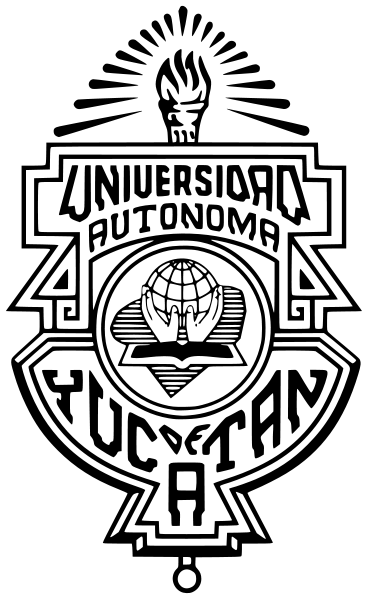
\includegraphics[scale=0.3]{UADY.png}
	\end{figure}}
	\vspace{0.7cm}
	{\Large\itshape Erick Al. Casanova Cortés\par}
	{\Large\itshape Matricula: 15014866\par}
	\vfill
	{\scshape\Large Docente\par
	Dra. María Milagrosa Pérez\par}
	\vfill
	{\Large{\bfseries Fecha de entrega: 7 Febrero 2021} }

	\vfill
	
\end{titlepage}

%-------------------------------------------------
%Inicio del documento
%-------------------------------------------------

\tableofcontents


\section{Introducción}

En el presente documento se relatará a manera de diario el transcurso de la cuarentena en práctica diaria de kundalini yoga. En este caso se eligió tanto un kriyas y una meditación para llevar a cabo durante la práctica. El kriya que se eligrió fue el \textit{Sat kriya}, por el hecho de que estaba la facilidad de seguirlo desde YouTube; por parte de la meditación se optó por una serie de meditaciones como se verá a lo largo del trayecto, las cuales tienen el nombre de \textit{Vipassana} y \textit{Anapanasati}, ya que estas dos son meditaciones que ya había llevado desde hace tiempo y realmente me resultan bastante gratificante.\\
Como pequeña descripción de las meditaciones, ya que no fueron vistas en el curso, \textit{Anapanasati} consiste en sólo observar la respiración y ser consiente de la misma en todo el momento, mientras \textit{Vipassana} es la observación de las sensaciones haciendo un barrido por todo el cuerpo.

%-------------------------------------------------
%Bitácora
%-------------------------------------------------

\chapter{Bitácora}

\section{Día 1}
	22/12/2020\\
	Hoy es mi primer día de práctica, terminé haciendo la práctica algo en la noche después de arreglar el cuarto y me sentí bastante bien, en sí la meditación se me hizo algo pesada pero logré hacer unos 20 minutos
	
\section{Día 2}
	23/12/2020\\
\section{Día 3}
\section{Día 4}
\section{Día 5}
\section{Día 6}
\section{Día 7}
\section{Día 8}
\section{Día 9}
\section{Día 10}
\section{Día 11}
\section{Día 12}
\section{Día 13}
\section{Día 14}
\section{Día 15}
\section{Día 16}
\section{Día 17}
\section{Día 18}
\section{Día 19}
\section{Día 20}
\section{Día 21}
\section{Día 22}
\section{Día 23}
\section{Día 24}
\section{Día 25}
\section{Día 26}
\section{Día 27}
\section{Día 28}
\section{Día 29}
\section{Día 30}
\section{Día 31}
\section{Día 32}
\section{Día 33}
\section{Día 34}
\section{Día 35}
\section{Día 36}
\section{Día 37}
\section{Día 38}
\section{Día 39}
\section{Día 40}

%-------------------------------------------------
%Final del documento
%-------------------------------------------------

\end{document}
